\chapter{Halting Problem}


\section{Halting Problem for Register Machines}
A register machine $H$ decides the halting problem if for all $e, a_1, \dots, a_n \in \mathbb{N}$:
\[\begin{matrix}
		\reglabel{0} = 0 & \reglabel{1} = e & \reglabel{2} = \ulcorner [a_1, \dots, a_n]\urcorner & \reglabel{3..} = 0 \\
	\end{matrix}\]
And where $H$ halt with the state as follows:
\[\reglabel{0} = \begin{cases}
		1 & \text{Register machine encoded as $e$ halts when started with $\reglabel{0} = 0, \reglabel{1} = a_1, \dots, \reglabel{n} = a_n$} \\
		0 & otherwise                                                                                                                        \\
	\end{cases}\]
We can prove that there is no such machine $H$ through a contradiction.
\begin{center}
    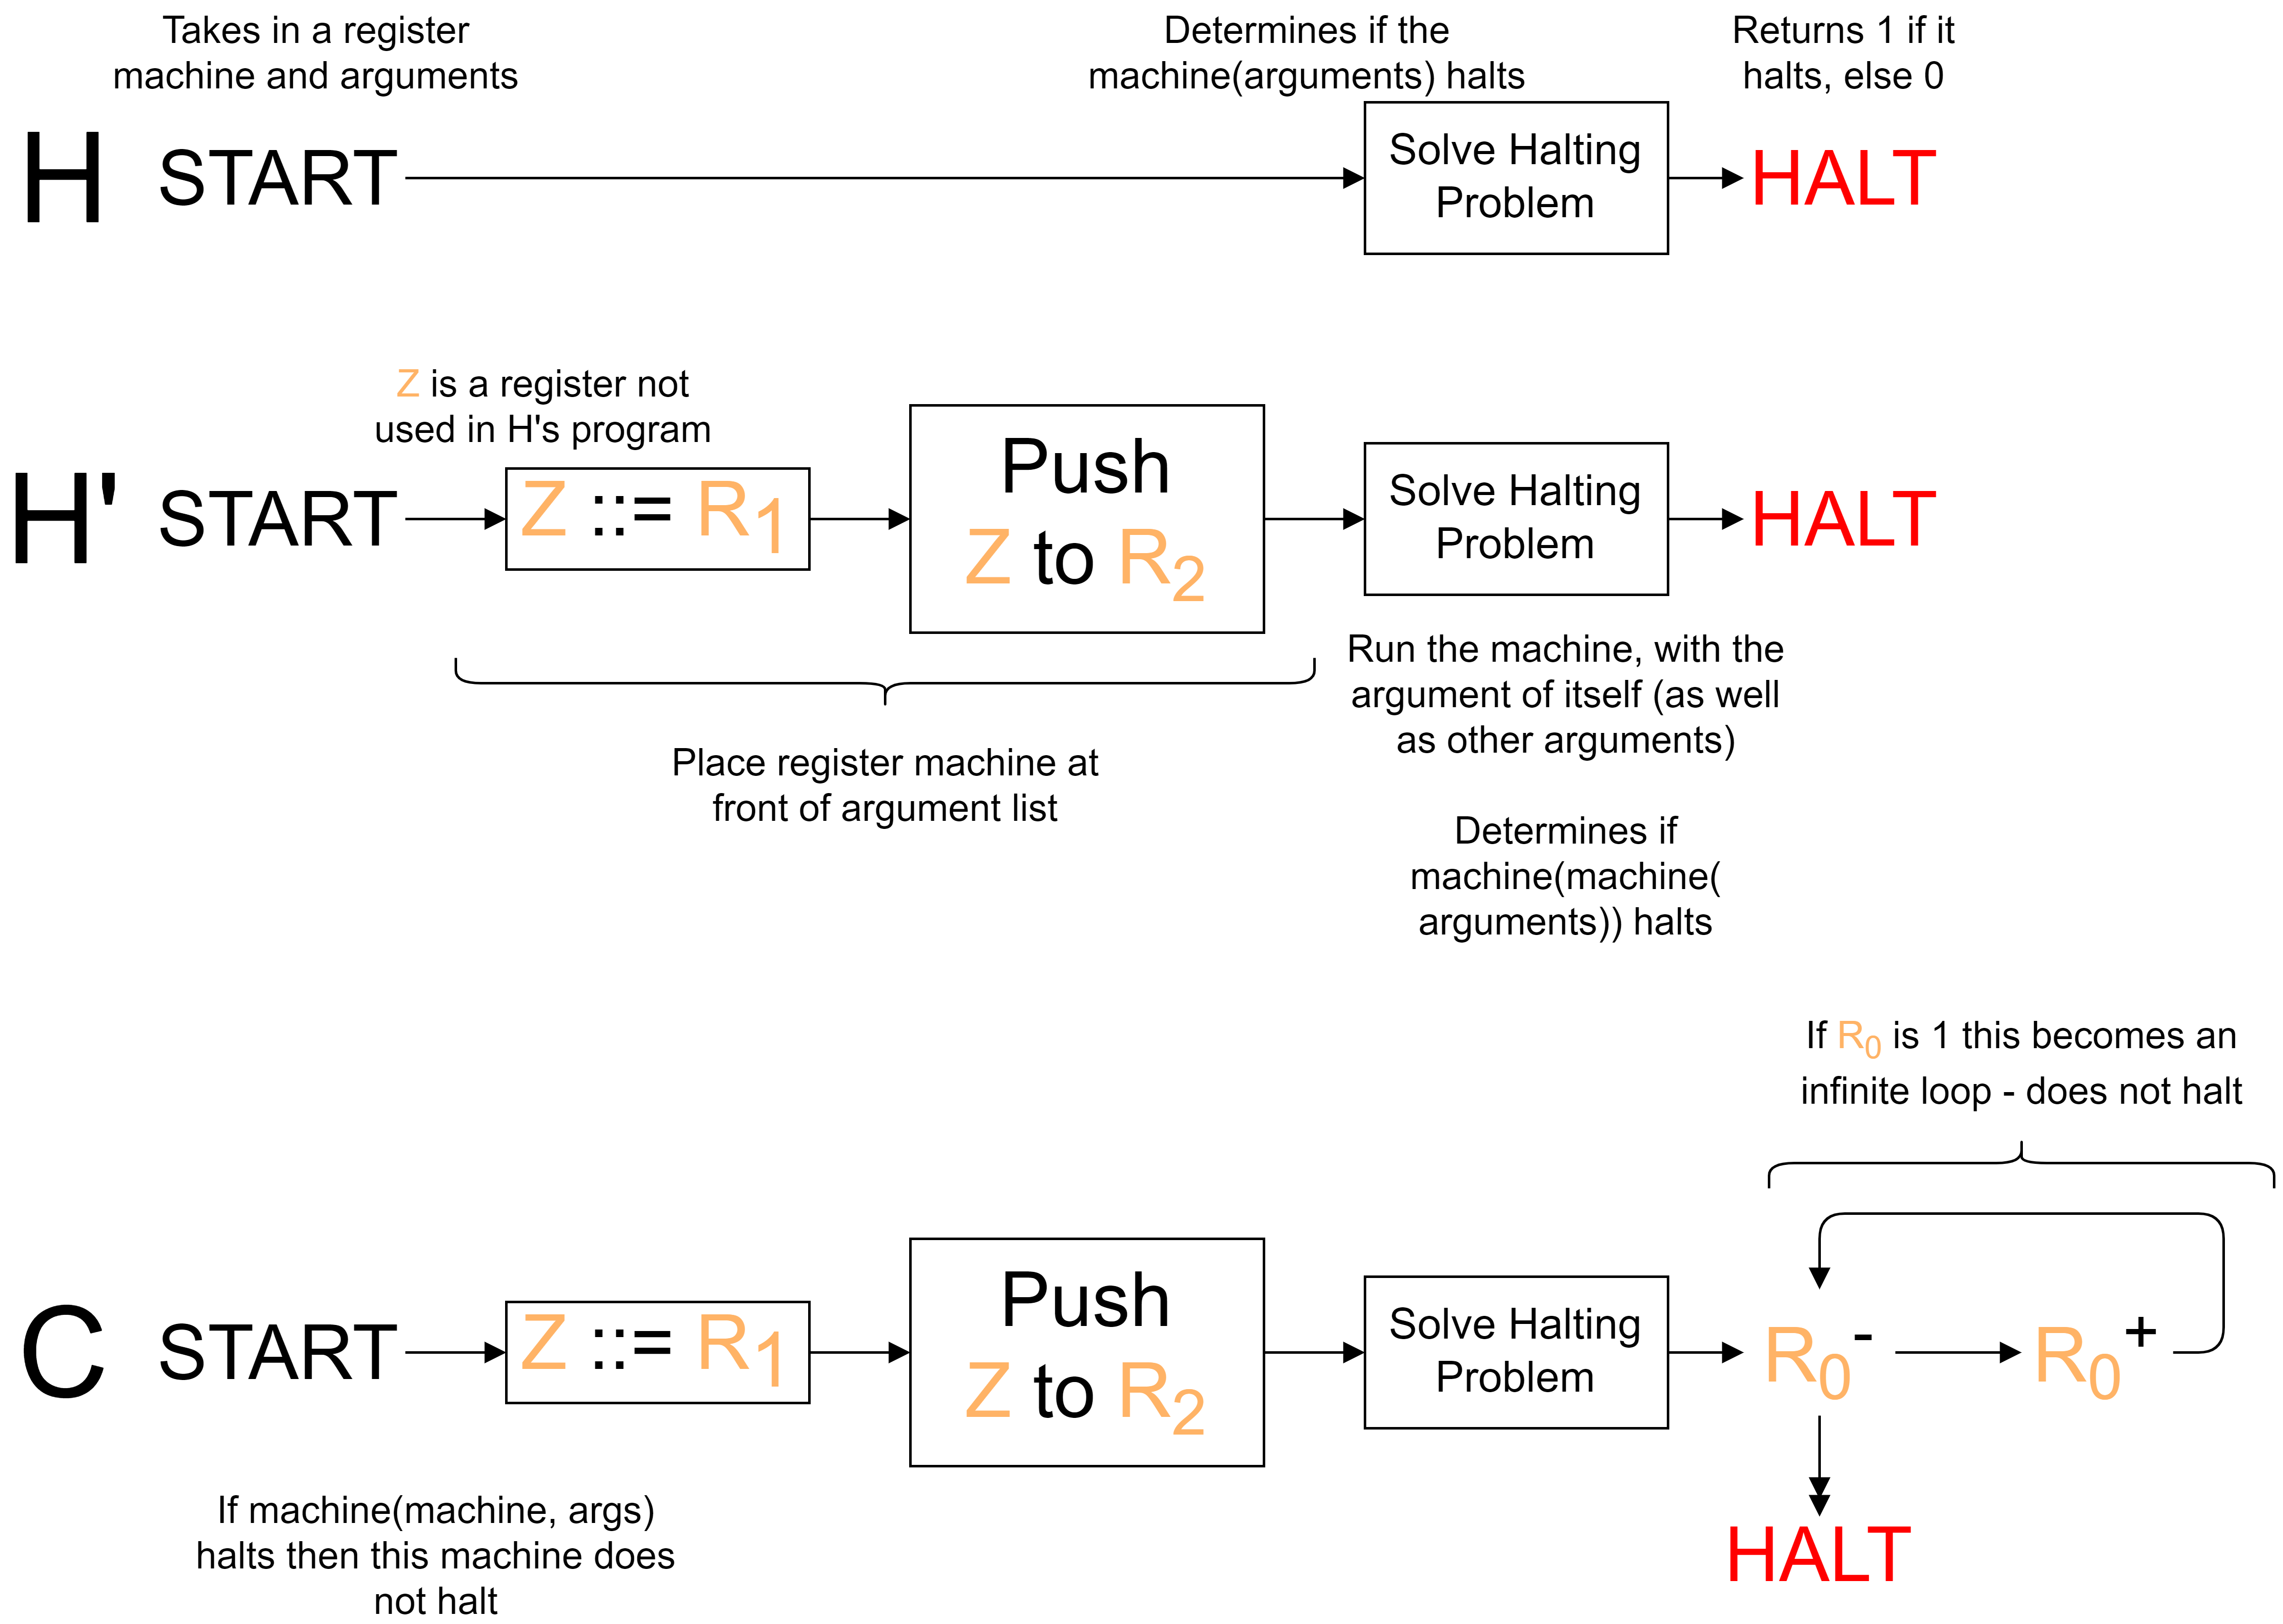
\includegraphics[width=0.9\textwidth]{halting_problem/images/halting_problem.drawio.png}
\end{center}
Hence when we run $C$ with the argument $C$ we get a contradiction.
\begin{center}
    \begin{tabular}{l p{.8\textwidth}}
        \textbf{$C(C)$ Halts} & Then $C$ with $\reglabel{1} = \ulcorner C \urcorner$ as an argument does not halt, which is a contradiction \\
        \textbf{$C(C)$ Does not Halt} & Then $C$ with $\reglabel{1} = \ulcorner C \urcorner$ as an argument halts, which is a contradiction \\
    \end{tabular}
\end{center}

\section{Computable Functions}
\subsection{Enumerating the Computable Functions}
\begin{definitionbox}{Onto (Surjective)}
    Each element in the codomain is mapped to by at least one element in the domain.
    \[\forall y \in Y. \  \exists x \in X. \  [f(x) = y] \Rightarrow f \text{ is onto}\]
\end{definitionbox}

For each $e \in \mathbb{N}$, $\varphi_e \in \mathbb{N} \rightharpoonup \mathbb{N}$ (partial function computed by $program(e)$):
\[\varphi_e(x) = y \Leftrightarrow program(e) \text{ with } \reglabel{0} = 0 \land \reglabel{1} = x \text{ halts with } \reglabel{0} = y\]
Hence for a given program $\in \mathbb{N}$ we can get the computable partial function of the program.
\[e \mapsto \varphi_e\]
Therefore the above mapping represents an \textit{onto/surjective} function from $\mathbb{N}$ to all computable partial functions from $\mathbb{N} \rightharpoonup \mathbb{N}$.

\subsection{Uncomputable Functions}
For $f: X \rightharpoonup Y$ (partial function from $X$ to $Y$):
\[\begin{split}
        f(x)\uparrow & \triangleq \neg \exists y \in Y . \ [f(x) = y] \\
        f(x)\downarrow & \triangleq  \exists y \in Y . \ [f(x) = y] \\
    \end{split}\]

Hence we can attempt to define a function to determine if a function halts.
\[f \in \mathbb{N} \rightharpoonup \mathbb{N} \triangleq \{(x,0) | \varphi_x(x)\uparrow\} \triangleq f(x) = \begin{cases}
		0         & \varphi_x(x)\uparrow   \\
		undefined & \varphi_x(x)\downarrow
	\end{cases}\]
However we run into the halting problem:
\\
\\ Assume $f$ is computable, then $f = \varphi_e$ for some $e \in \mathbb{N}$.

\begin{center}
    \begin{tabular}{l p{.8\textwidth}}
        \textbf{if $\varphi_e(e)\uparrow$} & by definition of $f$, $\varphi_e(e) = 0$ so $\varphi_e(e)\downarrow$ which is a contradiction \\
        \textbf{if $\varphi_e(e)\downarrow$} & by definition of $f$, $f(e)\uparrow$, and hence as $f = \varphi_e$, $\varphi_e\uparrow$ which is a contradiction \\
    \end{tabular}
\end{center}

Here we have ended up with the halting problem being uncomputable.

\subsection{Undecidable Set of Numbers}
Given a set $S \subseteq \mathbb{N}$, its characteristic function is:
\[\chi_S \in \mathbb{N} \to \mathbb{N} \ \ \chi_S(x) \triangleq \begin{cases}
		1 & x \in S     \\
		0 & x \not\in S \\
	\end{cases}\]
$S$ is \textit{register machine decidable} if its characteristic function is a register machine computable function.
\\
\\ $S$ is decidable iff there is a register machine $M$ such that for all $x \in \mathbb{N}$ when run with $\reglabel{0} = 0, \reglabel{1} = x$ and $\reglabel{2..} = 0$ it eventually halts with:
\[\reglabel{0} = 1 \Leftrightarrow x \in S \qquad \qquad \reglabel{0} = 1 x \not\in S \]
Hence we are effectively asking if a register machine exists that can determine if any number is in some set $S$.
\\
\\ We can then define subsets of $\mathbb{N}$ that are decidable/undecidable.

\subsubsection{The set of functions mapping $0$ is undecidable}
Given a set:
\[S_0 \triangleq \{e | \varphi_e(0)\downarrow\}\]
Hence we are finding the set of the indexes (numbers representing register machines) that halt on input $0$.
\\
\\ If such a machine exists, we can use it to create a register machine to solve the halting problem. Hence this is a contradiction, so the set is undecidable.

\subsubsection{The set of total functions is undecidable}
Take set $S_1 \subseteq \mathbb{N}$:
\[S_1 \triangleq \{e | \varphi_e\text{total function}\}\]
If such a register machine exists to compute $\chi_{S_1}$, we can create another register machine, simply checking $0$. Hence as from the previous example, there is no register machine to determine $S_0$, there is none to determine $S_1$.
